%% This is emulateapj reformatting of the AASTEX sample document
%%
%\documentclass[apj,twocolappendix,numberedappendix,appendixfloats]{emulateapj}
\documentclass[useAMS,usenatbib]{mnras}
\usepackage{showyourwork}

\usepackage{natbib}
%\bibliographystyle{apj}
\bibliographystyle{mnras}

\usepackage{tabu,booktabs}
\usepackage{amsmath}
\usepackage{xcolor}
\usepackage[english]{babel}
\usepackage{graphicx}
\usepackage{xspace}

\usepackage{longtable}
\usepackage{threeparttablex}
\usepackage{array}

% --- HACK to remove showyourwork abstract margin icon
\makeatletter
\def\abstract{\if@twocolumn
   \start@SFBbox\@abstract
 \else
   \@abstract
 \fi}
\def\endabstract{\if@twocolumn
   \endlist\finish@SFBbox
 \else
  \endlist
 \fi}
\makeatother
% ---

%\usepackage{pdflscape}

%%%%% AUTHORS - PLACE YOUR OWN MACROS HERE %%%%%

\def \etal {et~al.~}
\newcommand{\MKN}[1]{{\color{blue}{\bf MKN}:~ #1}}

\newcommand{\Rmax}{$R_{\rm max}$}
\newcommand{\Vmax}{$V_{\rm max}$}
\newcommand{\nPS}{$n_{\rm P\&S}$}
\newcommand{\nEin}{$n_{\rm E}$}
\newcommand{\amiga}{\texttt{AMIGA}}
\newcommand{\ahf}{\texttt{AHF}}
\newcommand{\mlapm}{\texttt{MLAPM}}
\newcommand{\hMpc}{{\ifmmode{h^{-1}{\rm Mpc}}\else{$h^{-1}$Mpc}\fi}}
\newcommand{\Mpc}{{\ifmmode{{\rm Mpc}}\else{Mpc}\fi}}
\newcommand{\hkpc}{{\ifmmode{h^{-1}{\rm kpc}}\else{$h^{-1}$kpc}\fi}}
\newcommand{\kpc}{{\ifmmode{ {\rm kpc} }\else{{\rm kpc}}\fi}}
\newcommand{\kms}{{\ifmmode{ {\rm km\,s^{-1}} }\else{ ${\rm km\,s^{-1}}$ }\fi}}
\newcommand{\hMsun}{{\ifmmode{h^{-1}{\rm {M_{\odot}}}}\else{$h^{-1}{\rm{M_{\odot}}}$}\fi}}
\newcommand{\Msun}{{\ifmmode{{\rm M}_{\odot}}\else{${\rm M}_{\odot}$}\fi}}
\newcommand{\Mhalo}{{\ifmmode{M_{\rm halo}}\else{$M_{\rm halo}$}\fi}}
\newcommand{\Rvir}{{\ifmmode{R_{\rm vir}}\else{$R_{\rm vir}$}\fi}}
\newcommand{\Mvir}{{\ifmmode{M_{\rm vir}}\else{$M_{\rm vir}$}\fi}}
\newcommand{\Mstar}{{\ifmmode{M_{\rm star}}\else{$M_{\rm star}$}\fi}}
\newcommand{\Vrot}{{\ifmmode{V_{\rm rot}}\else{$V_{\rm rot}$}\fi}}
\newcommand{\ltsima}{$\; \buildrel < \over \sim \;$}
\newcommand{\gtsima}{$\; \buildrel > \over \sim \;$}
\newcommand{\lsim}{\lower.5ex\hbox{\ltsima}}
\newcommand{\gsim}{\lower.5ex\hbox{\gtsima}}
\def\nbody{$N$-body}
\def\lesssim{\mathrel{\hbox{\rlap{\hbox{\lower4pt\hbox{$\sim$}}}\hbox{$<$}}}}
\def\gtrsim{\mathrel{\hbox{\rlap{\hbox{\lower4pt\hbox{$\sim$}}}\hbox{$>$}}}}
\newcommand{\new}[1]{\textbf{\textcolor{blue}{#1}}}
\newcommand{\problem}[1]{\textbf{\textcolor{red}{#1}}}
\newcommand{\Sec}[1]{Section~\ref{#1}}
\newcommand{\Eq}[1]{Eq.~(\ref{#1})}
\newcommand{\Fig}[1]{Fig.~\ref{#1}}
\newcommand{\beq}{\begin{equation}}
\newcommand{\eeq}{\end{equation}}
\def\beqa{\begin{eqnarray}}
\def\eeqa{\end{eqnarray}}
\def\LCDM{\ensuremath{\Lambda}CDM}
\def\LWDM{\ensuremath{\Lambda}WDM}
\def\head{ \vbox to 0pt{\vss \hbox to 0pt{\hskip 440pt\rm
      LA-UR-10-07069\hss} \vskip 25pt}}

%%UNITS
\def \kms {\ifmmode  \,\rm km\,s^{-1} \else $\,\rm km\,s^{-1}  $ \fi }
\def \kpc {\ifmmode  {\rm kpc}  \else ${\rm  kpc}$ \fi  }  
\def \hkpc {\ifmmode  {h^{-1}\rm kpc}  \else ${h^{-1}\rm kpc}$ \fi  }  
\def \hMpc {\ifmmode  {h^{-1}\rm Mpc}  \else ${h^{-1}\rm Mpc}$ \fi  }  
\def \Mpch {\ifmmode  {h^{-1}\rm Mpc}  \else ${h^{-1}\rm Mpc}$ \fi  }  
\def \Msun {\ifmmode {\rm M}_{\odot} \else ${\rm M}_{\odot}$ \fi} 
\def \hMsun {\ifmmode h^{-1}\,\rm M_{\odot} \else $h^{-1}\,\rm M_{\odot}$ \fi}

%%COSMOLOGY
\def \LCDM {\ifmmode \Lambda{\rm CDM} \else $\Lambda{\rm CDM}$ \fi}
\def \sig8 {\ifmmode \sigma_8 \else $\sigma_8$ \fi} 
\def \OmegaM {\ifmmode \Omega_{\rm m} \else $\Omega_{\rm m}$ \fi} 
\def \Omegab {\ifmmode \Omega_{\rm b} \else $\Omega_{\rm b}$ \fi} 
\def \OmegaL {\ifmmode \Omega_{\rm \Lambda} \else $\Omega_{\rm \Lambda}$\fi} 
\def \Deltavir {\ifmmode \Delta_{\rm vir} \else $\Delta_{\rm vir}$ \fi}
\def \rhocrit {\ifmmode \rho_{\rm crit} \else $\rho_{\rm crit}$ \fi}
\def \rhou {\ifmmode \rho_{\rm u} \else $\rho_{\rm u}$ \fi}
\def \zc {\ifmmode z_{\rm c} \else $z_{\rm c}$ \fi}

\def\lcdm{\ensuremath{\Lambda\textrm{CDM}}\xspace}  
\def\omegam{\ensuremath{\Omega_\textrm{m}}\xspace}
\def\omegal{\ensuremath{\Omega_\Lambda}\xspace}
\def\omegab{\ensuremath{\Omega_\textrm{b}}\xspace}
\def\omegar{\ensuremath{\Omega_\textrm{r}}\xspace}
%%%%% AUTHORS - PLACE YOUR OWN MACROS HERE %%%%%

%\usepackage{tabu,booktabs}

\def\aj{AJ}%
         % Astronomical Journal
\def\actaa{Acta Astron.}%
         % Acta Astronomica
\def\araa{ARA\&A}%
         % Annual Review of Astron and Astrophys
\def\apj{ApJ}%
         % Astrophysical Journal
\def\apjl{ApJ}%
         % Astrophysical Journal, Letters
\def\apjs{ApJS}%
         % Astrophysical Journal, Supplement
\def\ao{Appl.~Opt.}%
         % Applied Optics
\def\apss{Ap\&SS}%
         % Astrophysics and Space Science
\def\aap{A\&A}%
         % Astronomy and Astrophysics
\def\aapr{A\&A~Rev.}%
         % Astronomy and Astrophysics Reviews
\def\aaps{A\&AS}%
         % Astronomy and Astrophysics, Supplement
\def\azh{AZh}%
         % Astronomicheskii Zhurnal
\def\baas{BAAS}%
         % Bulletin of the AAS
\def\bac{Bull. astr. Inst. Czechosl.}%
         % Bulletin of the Astronomical Institutes of Czechoslovakia
\def\caa{Chinese Astron. Astrophys.}%
         % Chinese Astronomy and Astrophysics
\def\cjaa{Chinese J. Astron. Astrophys.}%
         % Chinese Journal of Astronomy and Astrophysics
\def\icarus{Icarus}%
         % Icarus
\def\jcap{J. Cosmology Astropart. Phys.}%
         % Journal of Cosmology and Astroparticle Physics
\def\jrasc{JRASC}%
         % Journal of the RAS of Canada
\def\mnras{MNRAS}%
         % Monthly Notices of the RAS
\def\memras{MmRAS}%
         % Memoirs of the RAS
\def\na{New A}%
         % New Astronomy
\def\nar{New A Rev.}%
         % New Astronomy Review
\def\pasa{PASA}%
         % Publications of the Astron. Soc. of Australia
\def\pra{Phys.~Rev.~A}%
         % Physical Review A: General Physics
\def\prb{Phys.~Rev.~B}%
         % Physical Review B: Solid State
\def\prc{Phys.~Rev.~C}%
         % Physical Review C
\def\prd{Phys.~Rev.~D}%
         % Physical Review D
\def\pre{Phys.~Rev.~E}%
         % Physical Review E
\def\prl{Phys.~Rev.~Lett.}%
         % Physical Review Letters
\def\pasp{PASP}%
         % Publications of the ASP
\def\pasj{PASJ}%
         % Publications of the ASJ
\def\qjras{QJRAS}%
         % Quarterly Journal of the RAS
\def\rmxaa{Rev. Mexicana Astron. Astrofis.}%
         % Revista Mexicana de Astronomia y Astrofisica
\def\skytel{S\&T}%
         % Sky and Telescope
\def\solphys{Sol.~Phys.}%
         % Solar Physics
\def\sovast{Soviet~Ast.}%
         % Soviet Astronomy
\def\ssr{Space~Sci.~Rev.}%
         % Space Science Reviews
\def\zap{ZAp}%
         % Zeitschrift fuer Astrophysik
\def\nat{Nature}%
         % Nature
\def\iaucirc{IAU~Circ.}%
         % IAU Cirulars
\def\aplett{Astrophys.~Lett.}%
         % Astrophysics Letters
\def\apspr{Astrophys.~Space~Phys.~Res.}%
         % Astrophysics Space Physics Research
\def\bain{Bull.~Astron.~Inst.~Netherlands}%
         % Bulletin Astronomical Institute of the Netherlands
\def\fcp{Fund.~Cosmic~Phys.}%
         % Fundamental Cosmic Physics
\def\gca{Geochim.~Cosmochim.~Acta}%
         % Geochimica Cosmochimica Acta
\def\grl{Geophys.~Res.~Lett.}%
         % Geophysics Research Letters
\def\jcp{J.~Chem.~Phys.}%
         % Journal of Chemical Physics
\def\jgr{J.~Geophys.~Res.}%
         % Journal of Geophysics Research
\def\jqsrt{J.~Quant.~Spec.~Radiat.~Transf.}%
         % Journal of Quantitiative Spectroscopy and Radiative Trasfer
\def\memsai{Mem.~Soc.~Astron.~Italiana}%
         % Mem. Societa Astronomica Italiana
\def\nphysa{Nucl.~Phys.~A}%
         % Nuclear Physics A
\def\physrep{Phys.~Rep.}%
         % Physics Reports
\def\physscr{Phys.~Scr}%
         % Physica Scripta
\def\planss{Planet.~Space~Sci.}%
         % Planetary Space Science
\def\procspie{Proc.~SPIE}%
         % Proceedings of the SPIE

%\newcommand\lcdm{\ifluatex \char"039B CDM\else\ifxetex\char"039B CDM \else%
%    \ensuremath{$\Lambda$\textrm{CDM}}\fi\xspace}

\def\head{ .ps \vbox to 0pt{\vss \hbox to 0pt{\hskip 440pt\rm
      LA-UR-10-07069\hss} \vskip 25pt}} 

\def \spose#1{\hbox  to 0pt{#1\hss}}  
\def \lta{\mathrel{\spose{\lower 3pt\hbox{$\sim$}}\raise 2.0pt\hbox{$<$}}}
\def \gta{\mathrel{\spose{\lower 3pt\hbox{$\sim$}}\raise 2.0pt\hbox{$>$}}}

\def\lcdm{\ensuremath{\Lambda\textrm{CDM}}\xspace}
    
\def\omegam{\ensuremath{\Omega_\textrm{m}}\xspace}
\def\omegal{\ensuremath{\Omega_\Lambda}\xspace}
\def\omegab{\ensuremath{\Omega_\textrm{b}}\xspace}
\def\omegar{\ensuremath{\Omega_\textrm{r}}\xspace}


%%%%%%%%%%%%%%%%%%%%%%%%%%%%%%%%%%%%%%%%%%%%%%%%%%%
\title[Early massive accretion events in a MW-mass galaxy]{The influence of massive early merger events on the chemo-dynamics of galaxy discs}

\author[T. Buck] {Tobias Buck$^{1,2}$\thanks{E-mail: tobias.buck@iwr-uni-heidelberg.de.de}, Aura Obreja$^{3}$, \etal \\  %Andrea V. Macci\`o$^{4,5}$, \etal \\
%, Aaron A. Dutton$^{2}$, Andrea V. Macci\`o$^{2,1}$\\
%
$^1$Universit\"at Heidelberg, Interdisziplin\"ares Zentrum f\"ur Wissenschaftliches Rechnen, Im Neuenheimer Feld 205, D-69120 Heidelberg, Germany\\
$^2$Universit\"at Heidelberg, Zentrum f\"ur Astronomie, Institut f\"ur Theoretische Astrophysik, Albert-Ueberle-Straße 2, 69120 Heidelberg, Germany\\
$^3$Universit\"ats-Sternwarte M\"unchen, Scheinerstraße 1, D-81679 M\"unchen, Germany%\\
%$^4$New York University Abu Dhabi, PO Box 129188, Saadiyat Island, Abu Dhabi, United Arab Emirates\\
%$^5$Max-Planck-Institut f\"ur Astronomie, K\"onigstuhl 17, 69117 Heidelberg, Germany\\
}

\setlength{\topmargin}{-1.2cm}

\begin{document}

\date{Accepted XXXX . Received XXXX; in original form XXXX}

\pagerange{\pageref{firstpage}--\pageref{lastpage}} \pubyear{2022}

\maketitle

\label{firstpage}


\begin{abstract}
awesome science! keep on reading and cite me! 
\end{abstract}

%%%%%%%%%%%%%%%%%%%%%%%%%%%%%%%%%%%%%%%%%%%%%%%%%%%
\noindent
\begin{keywords}

Galaxy: structure --- Galaxy: evolution --- Galaxy: kinematics and dynamics --- galaxies:
  formation --- Galaxy: disk --- methods: numerical
 \end{keywords}

%%%%%%%%%%%%%%%%%%%%%%%%%%%%%%%%%%%%%%%%%%%%%%%%%%%


%%%%%%%%%%%%%%%%%%%%%%%%%%%%%%%%%%%%%%%%%%%%%%%%%%%
\section{Introduction} \label{sec:introduction}
%%%%%%%%%%%%%%%%%%%%%%%%%%%%%%%%%%%%%%%%%%%%%%%%%%%



%%%%%%%%%%%%%%%%%%%%%%%%%%%%%%%%%%%%%%%%%%%%%%%%%%%
\section{Methods} \label{sec:simulation}
%%%%%%%%%%%%%%%%%%%%%%%%%%%%%%%%%%%%%%%%%%%%%%%%%%%

\begin{figure}
    \script{half_mass_radius_gas.py}
    \begin{centering}
        \includegraphics[width=\linewidth]{figures/279e12_gas_size.pdf}
        \caption{
            Half mass radius of the cold gas as a function of time. The sharp increases in the cold gas size around 2 Gyr and 9 Gyr indicate the influence of massive gas rich merger events on the galaxy. The addition of fresh cold gas leads to a sudden increase in cold gas half mass size.
        }
        \label{fig:half_mass}
    \end{centering}
\end{figure}


\begin{figure}
    \begin{centering}
        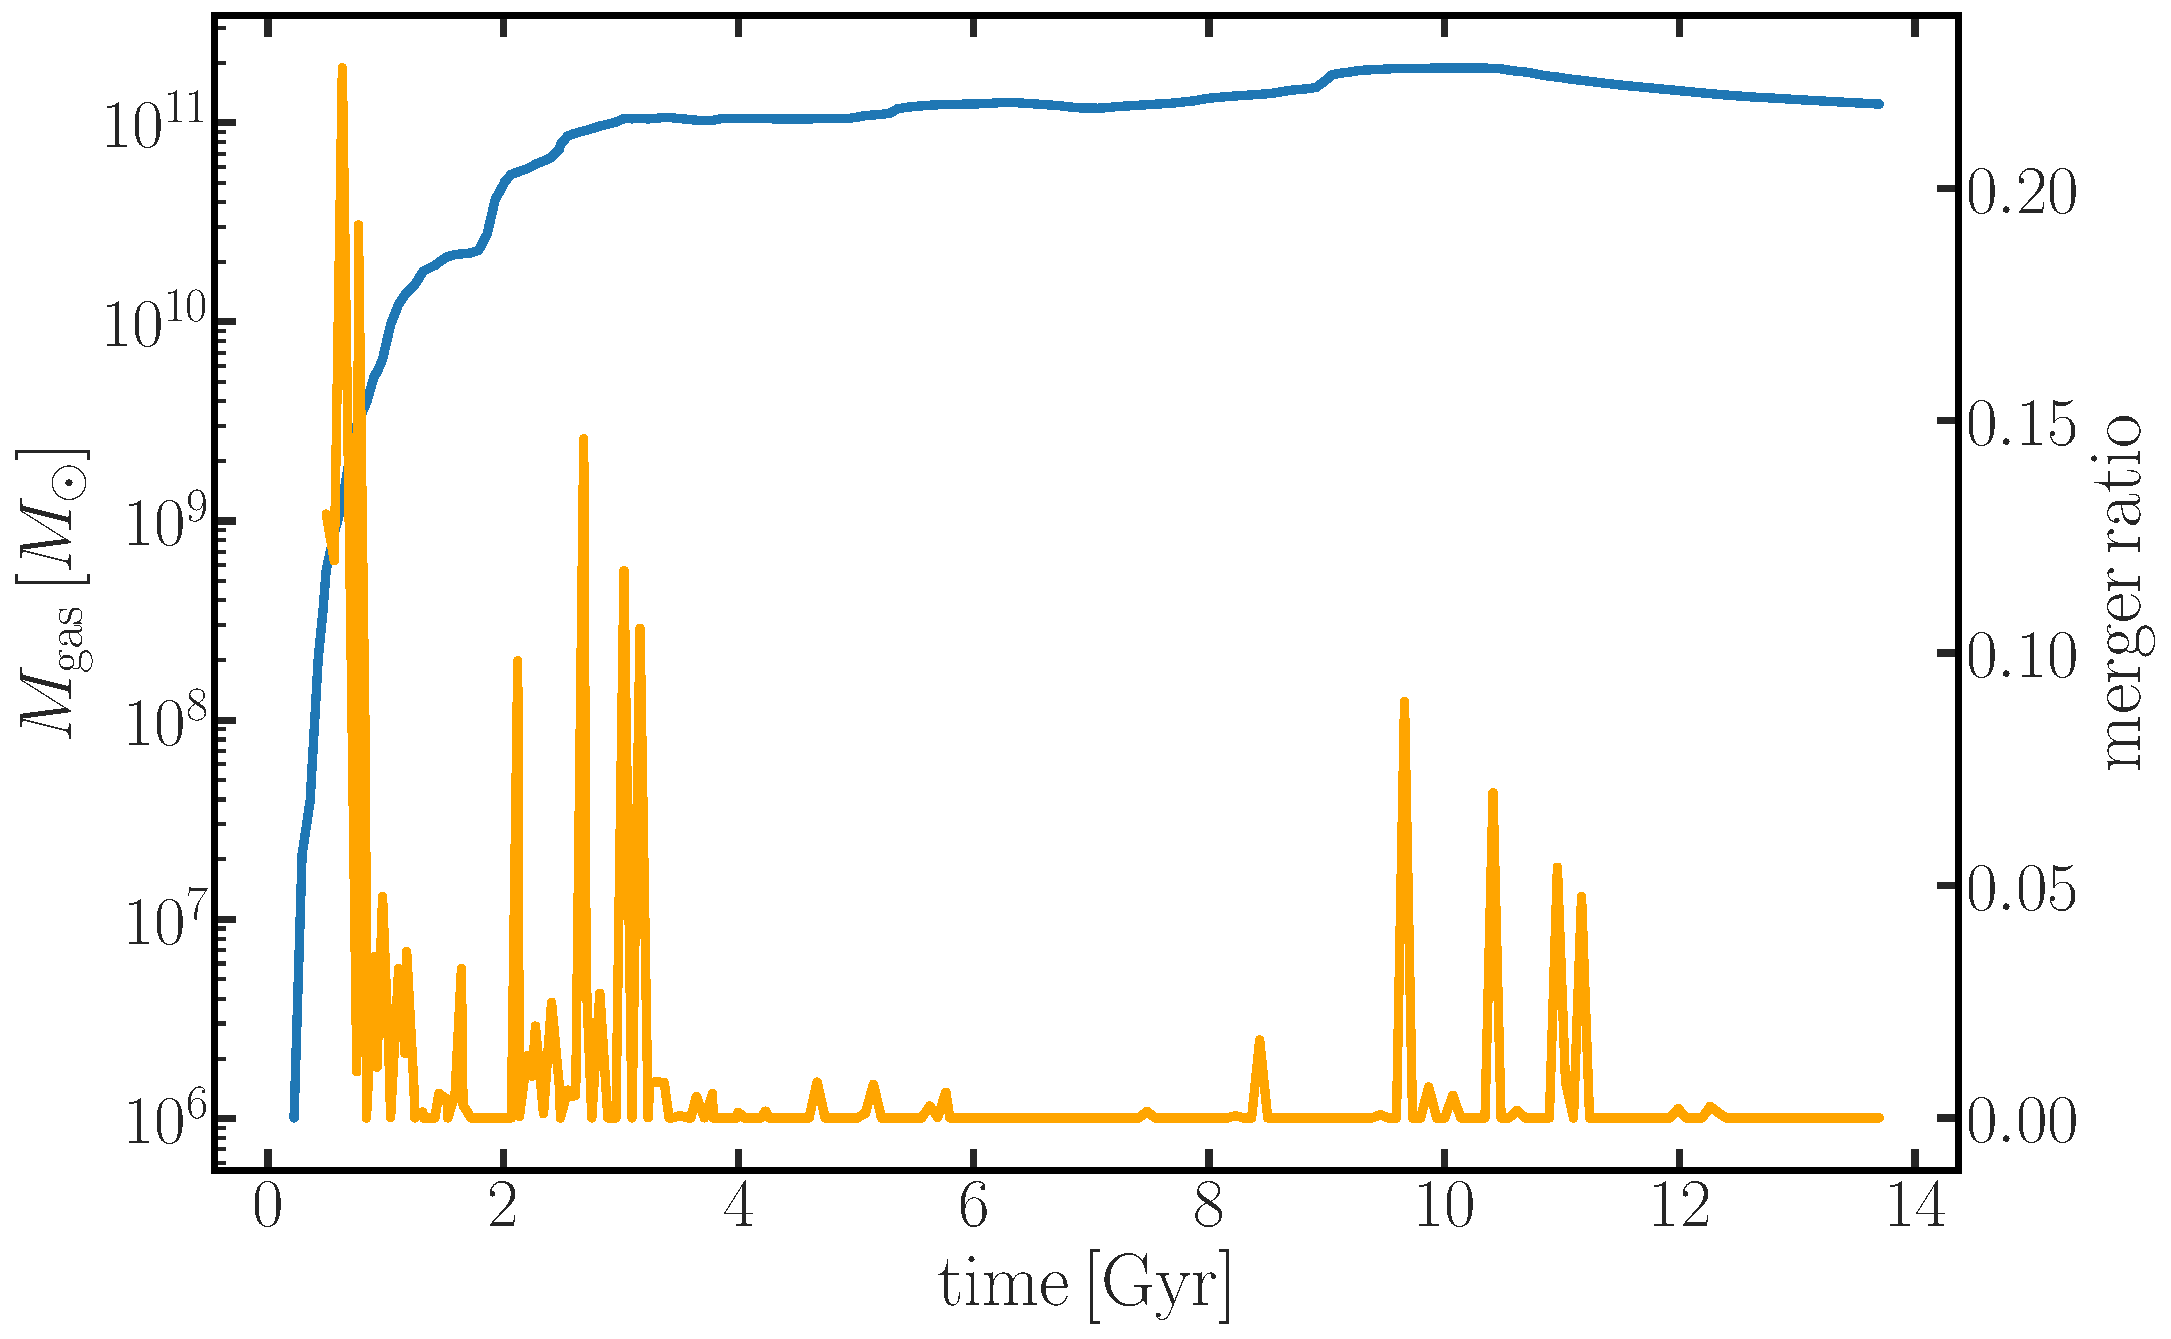
\includegraphics[width=\linewidth]{figures/279e12_merger_ratio_gas.pdf}
        \caption{Gas mass (blue line, left axis) and merger ratio (orange line, right axis) as a function of time. We identify gas rich mergers that contribute around 10\% of gas to the main galaxy between times of 2-4 Gyr and a late time merger starting around 9.5 Gyr that contributes 10\% of gas and continues for several pericenter passages and goes on for $\sim2$ Gyr.
        }
        \label{fig:merger_ratio}
    \end{centering}
\end{figure}

\begin{figure}
    \script{half_mass_radius_metal_gradient.py}
    \begin{centering}
        \includegraphics[width=\linewidth]{figures/half_mass_radius_metal_gradient.pdf}
        \caption{
            Half mass radius of the cold gas (orange line, right axis) and the metallicity gradient (blue line, left axis) as a function of time. The sharp increases in the cold gas size around the times of gas rich mergers coincide with a sudden steepening of the metallicity gradient of $\sim0.02$ dex/kpc. The addition of relatively unenriched cold gas by the merging satellite leads to a sudden increase of the star-forming cold gas  mass in the outskirts of the galaxies while the central parts are unaffected. This steepens the gradient.
        }
        \label{fig:half_mass}
    \end{centering}
\end{figure}

\begin{figure}
    \script{gas_profile.py}
    \begin{centering}
        \includegraphics[width=\linewidth]{figures/2.79e12_gas_profile_2d.pdf}
        \caption{
            Surface density profile of the cold gas before and after the two merger events. Outside of a radius of 5 kpc the merging satellites contribute cold gas up to a factor of 4 in surface density.
        }
        \label{fig:surf_den}
    \end{centering}
\end{figure}

\begin{figure}
    \script{v_phi.py}
    \begin{centering}
        \includegraphics[width=\linewidth]{figures/2.79e12_v_phi_gas.pdf}
        \caption{
            Histogram of the cold gas velocity in the disk plane, $v_\phi$, before and after the merger. The peak of the $v_\phi$ distribution shifts from 73 km/s before the merger to 140 km/s after the merger, almost doubling the rotation speed of the cold gas disk.
        }
        \label{fig:v_phi}
    \end{centering}
\end{figure}


\begin{figure*}
    \script{mdf.py}
    \begin{centering}
        \includegraphics[width=\linewidth]{figures/2.79e12_mdf_gas.pdf}
        \caption{
            Metallicity distribution function of the main galaxy and the merging satellite shortly before coalescence for all three merger events. Filled histograms show the gaseous MDF while steps show the MDF for stars. In any case, the gas metallicity of the satellite is $\sim0.5-0.75$ dex lower that the main galaxy's gas metallicity.
        }
        \label{fig:mdf}
    \end{centering}
\end{figure*}


\begin{figure*}
    \script{feh_gradient.py}
    \begin{centering}
        \includegraphics[width=\linewidth]{figures/feh_gradient.pdf}
        \caption{
            Metallicity gradient of the cold gas disk during the merger events. We find that the contribution of additional metal poor gas lowers the metallicity in the outskirts of the disk effectively steepening the metallicity gradient by $\sim 0.1$ dex.
        }
        \label{fig:feh_grad}
    \end{centering}
\end{figure*}







%%%%%%%%%%%%%%%%%%%%%%%%%%%%%%%%%%%%%%%%%%%%%%%%%%%
\section{Results} \label{sec:results}
%%%%%%%%%%%%%%%%%%%%%%%%%%%%%%%%%%%%%%%%%%%%%%%%%%%


\begin{figure*}
    \script{age_feh.py}
    \begin{centering}
        \includegraphics[width=\linewidth]{figures/2.79e12_age_metallicity_grid.pdf}
        \caption{
            Age-metallicity relation.
        }
        \label{fig:age_feh}
    \end{centering}
\end{figure*}

\begin{figure*}
    \script{feh_ofe.py}
    \begin{centering}
        \includegraphics[width=\linewidth]{figures/2.79e12_feh_ofe_grid.pdf}
        \caption{
            Oxygen vs. metallicity.
        }
        \label{fig:ofe_feh}
    \end{centering}
\end{figure*}







\subsection{some different elements [X/Fe] vs. [Fe/H]}
do different elements give us insight into different formation epochs of the MW?
detailed galactic archeology is left for future work.

\subsection{relative contribution of different enrichment channels in L* galaxies: SNII vs. AGB vs. SNIa}


%%%%%%%%%%%%%%%%%%%%%%%%%%%%%%%%%%%%%%%%%%%%%%%%%%%
\section{Conclusion}
\label{sec:conclusion}
%%%%%%%%%%%%%%%%%%%%%%%%%%%%%%%%%%%%%%%%%%%%%%%%%%%



Our results are summarized as follows:
\begin{itemize}
%
\item 

\end{itemize}



%%%%%%%%%%%%%%%%%%%%%%%%%%%%%%%%%%%%%%%%%%%%%%%%%%%
\section*{acknowledgments}
%\section*{Acknowledgments}
%%%%%%%%%%%%%%%%%%%%%%%%%%%%%%%%%%%%%%%%%%%%%%%%%%%
TB's contribution to this project was made possible by funding from the Carl Zeiss Foundation. TB gratefully acknowledges the Gauss Centre for Supercomputing e.V. (www.gauss-centre.eu) for funding this project by providing computing time on the GCS Supercomputer SuperMUC at Leibniz Supercomputing Centre (www.lrz.de). This research was carried out on the High Performance Computing resources at New York University Abu Dhabi.
This research made use of the {\sc{pynbody}} \citet{pynbody} package to analyze the simulations and used the {\sc{python}} package {\sc{matplotlib}} \citep{matplotlib} to display all figures in this work. Data analysis for this work made intensive use of the {\sc{python}} library {\sc{SciPy}} \citep{scipy}, in particular {\sc{NumPy and IPython}} \citep{numpy,ipython}. The article has been typeset using showyourwork! by \citet{Luger2021}.


\bibliography{bib.bib}

\appendix

\section{Rotation velocity of stars}

\begin{figure}
    \script{v_phi_stars.py}
    \begin{centering}
        \includegraphics[width=\linewidth]{figures/2.79e12_v_phi_stars.pdf}
        \caption{
            Same as Fig.~\ref{fig:v_phi} but for the stellar rotation velocity in the disk plane, $v_\phi$, before and after the merger. The peak of the $v_\phi$ distribution shifts from 27 km/s before the merger to 66 km/s after the merger, more than doubling the rotation speed of the stellar disk.
        }
        \label{fig:v_phi_stars}
    \end{centering}
\end{figure}

\section{Oxygen abundance distribution}

\begin{figure*}
    \script{mdf_oxygen.py}
    \begin{centering}
        \includegraphics[width=\linewidth]{figures/2.79e12_mdf_oxygen_gas.pdf}
        \caption{
            Same as Fig.~\ref{fig:mdf} but for the oxygen abundance. Filled histograms show the gaseous oxygen abundance distribution while steps show the one for stars. The gas oxygen abundance of the satellite is  $\sim0.1$ dex lower that the main galaxy's gas oxygen abundance.
        }
        \label{fig:mdf_oxygen}
    \end{centering}
\end{figure*}

\label{lastpage}
\end{document}

